\hypertarget{index_secScope}{}\section{Scope}\label{index_secScope}
This interface must be implemented by an application server (A\-S) or replication framework (R\-F) to receive sensor data from a sensor aggregation system (S\-A\-S). In addition, it is used to pass on sensor data from the replication framework (R\-F) to the appserver (A\-S).  
\begin{DoxyImage}
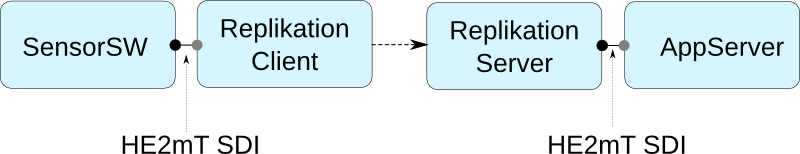
\includegraphics{interfaces.png}
\caption{width=1.0}
\end{DoxyImage}
\hypertarget{index_secGeneral}{}\section{General}\label{index_secGeneral}
All functions of this abstract class need to be implemented in order to receive sensor data. The functions of \hyperlink{classgeneric_param_interface}{generic\-Param\-Interface} need not be implemented. However, \hyperlink{classgeneric_param_interface}{generic\-Param\-Interface} can be used to expose a parameter interface that allows the sensor aggregation system to modify certain values of the application server. It is for debugging purposes, only. On java, \hyperlink{classgeneric_param_interface}{generic\-Param\-Interface} needs not to be implemented.

The interface is used as follows\-:
\begin{DoxyItemize}
\item First, the application using it calls \hyperlink{classhe2mt_s_d_i_a6a3b5da850e0571bc4a8c8e0de7ad9e8}{he2mt\-S\-D\-I\-::init()}
\item Then, it calls \hyperlink{classhe2mt_s_d_i_ae5212f96e535b795b11fd34a89a3d616}{he2mt\-S\-D\-I\-::authorize()}, providing authentication/authorization credentials. If no authentication/authorization is needed, the class implementing the interface can safely ignore all paramters and do nothing.\par

\item Then, data can be transferred via the interface by calling he2mt\-S\-D\-I\-::set\-Data()
\end{DoxyItemize}

When everything is done, the application can call \hyperlink{classhe2mt_s_d_i_a7f9d573e91544cc1436dab6bf1a889cf}{he2mt\-S\-D\-I\-::disconnect()} to stop being authenticated.\hypertarget{index_secSlots}{}\section{Data Slots}\label{index_secSlots}
The interface defines data slots. Data slots are virtual channels that an application can read from or write to. The interface is unidirectional, meaning a class implementing the interface can only read from a data slot (by implementing set\-Sensor\-Data), whereas the application using it (S\-A\-S or R\-F) can write to this data slot by calling \hyperlink{classhe2mt_s_d_i_a775fcd2c08e923050b76aa750895a983}{he2mt\-S\-D\-I\-::set\-Sensor\-Data()}. read more\-: \hyperlink{he2mt_s_d_i_data_slots_8h}{he2mt\-S\-D\-I\-Data\-Slots.\-h} \hypertarget{index_secSample}{}\section{Sample Program}\label{index_secSample}
The following code would use the interface correctly\-:

\#include \char`\"{}implementations/he2mt\-S\-D\-I\-Rest.\-hpp\char`\"{} \par
 int main()\{\par
 float values\mbox{[}6\mbox{]} = \{1,2,3,4,5,6\};\par
 uint32\-\_\-t activity = H\-E2\-M\-T\-\_\-\-S\-D\-I\-\_\-\-D\-A\-T\-A\-\_\-\-S\-L\-O\-T\-\_\-\-A\-C\-T\-I\-V\-I\-T\-Y\-\_\-\-V\-A\-L\-U\-E\-\_\-\-W\-A\-L\-K\-I\-N\-G;\par
 he2mt\-S\-D\-I\-Rest r;\par
 r.\-init();\par
 if(r.\-authorize(\char`\"{}id\char`\"{},\char`\"{}secret\char`\"{},\char`\"{}he2mt\-\_\-user\char`\"{},\char`\"{}he2mt\-\_\-user\char`\"{}))\{\par
 r.\-set\-Sensor\-Data(H\-E2\-M\-T\-\_\-\-S\-D\-I\-\_\-\-D\-A\-T\-A\-\_\-\-S\-L\-O\-T\-\_\-\-A\-C\-T\-I\-V\-I\-T\-Y,\char`\"{}0\char`\"{},\char`\"{}0\char`\"{},0.\-01,1,\&activity);\par
 r.\-set\-Sensor\-Data(H\-E2\-M\-T\-\_\-\-S\-D\-I\-\_\-\-D\-A\-T\-A\-\_\-\-S\-L\-O\-T\-\_\-\-R\-A\-W\-A\-C\-C,\char`\"{}0\char`\"{},\char`\"{}0\char`\"{},0.\-01,2,\&values);\par
 \}\par
 r.\-disconnect();\par
 \}\par
 